%
% =============================================================================
% Documentdefinition  beginns here
% =============================================================================

\documentclass[
10pt, % Schriftgrösse
a4paper, % A4 Papier
%%%%%%%% BCOR25mm, % Absoluter Wert der Bindekorrektur, z.B. BCOR1cm
BCOR15mm, % Absoluter Wert der Bindekorrektur, z.B. BCOR1cm
DIV14, % Satzspiegel festlegen siehe
       % http://www.ctex.org/documents/packages/nonstd/koma-script.pdf
footsepline = false, % Trennlinie zwischen Textkörper und Fußzeile
                     % bei normalen Seiten
headsepline, % Trennlinie zwischen Kopfzeile und Textkörper
             % bei normalen Seiten
oneside,
%%%%%%%% twoside, % Zweiseitig
openright,
parskip=half, % Europäischer Satz mit Abstand zwischen den Absätzen
abstracton, % inkl. Abstract
listof=totocnumbered, % Abb.- und Tab.verzeichnis im Inhaltsverzeichnis
bibliography=totocnumbered % Lit.zeichnis in Inhaltsverzeichnis aufnehmen
]{scrreprt}


\usepackage[left=2.5cm,right=2cm,top=3cm,bottom=3cm]{geometry}

\usepackage[
automark,
%plainheadsepline, % Trennlinie zwischen Textkörper und Kopfzeile
                   % bei Chapter Seiten, siehe headsepline, scrreprt
%plainfootsepline  % Trennlinie zwischen Textkörper und Fußzeile
                   % bei Chapter Seiten, siehe footsepline, scrreprt
]{scrpage2} % Gestaltung von kopf- und Fußzeile

\usepackage[ngerman]{babel}

\usepackage[ngerman]{translator}

\usepackage{tocbasic}


\usepackage{helvet} % Helvetica (sans-serif), ähnlich Arial
\renewcommand{\familydefault}{\sfdefault}

% Use utf-8 encoding for foreign characters
\usepackage[utf8]{inputenc}

\usepackage{lmodern} % Latin Modern

% \usepackage[applemac]{inputenc}
\usepackage[T1]{fontenc}

% Setup for fullpage use
%\usepackage{fullpage}

% Silbentrennung kann unterdrückt werden
\usepackage{hyphenat}

%1.5 Zeilenabstand
\usepackage[onehalfspacing]{setspace}

% Schöne Schriften für PDF-Dateien
\usepackage{ae}

% Tradmark
\def\TTra{\textsuperscript{\texttrademark}}

% Festlegung des Seitenstils (scrpage2)
\pagestyle{scrheadings}
\clearscrheadfoot
\automark[section]{chapter}

%\lehead{\sffamily\upshape\headmark}
%\cehead{}
%\rehead{}
%\lefoot[\pagemark]{\upshape \pagemark}
%\cefoot{}
%\refoot{}
\lohead{\sffamily\upshape\leftmark}
%\cohead{}

%\rohead{\sffamily\upshape\leftmark}
\lofoot{}
\cofoot{}
\rofoot[\pagemark]{\scshape \pagemark}

% Running Headers and footers
%\usepackage{fancyhdr}
%\setlength{\headheight}{15pt}

%\pagestyle{fancy}
%\renewcommand{\chaptermark}[1]{\markboth{\thechapter\ #1}{}}
%\renewcommand{\sectionmark}[1]{\markright{\thesection\ #1}{}}

%\fancyhf{}
%\fancyfoot[RE,LO]{\thepage}
%\fancyhead[LO]{\textit{\nouppercase{\leftmark}}}
%\fancyhead[RE]{\textit{\nouppercase{\rightmark}}}

%\renewcommand{\headrulewidth}{0.5pt}
%\renewcommand{\footrulewidth}{0pt}

%\fancypagestyle{plain}{%
%\fancyhf{}%
%\fancyfoot[RE,LO]{\thepage}
%\renewcommand{\headrulewidth}{0pt}
%\renewcommand{\footrulewidth}{0pt}
%}

%\setlength{\footskip}{1cm}

%\setlength{\headsep}{1.5cm}
%\addtolength{\textheight}{-1.5cm}

% Multipart figures
%\usepackage{subfigure}

% More symbols
%\usepackage{amsmath}
%\usepackage{amssymb}
%\usepackage{latexsym}

% Surround parts of graphics with box
\usepackage{boxedminipage}

\usepackage[svgnames]{xcolor}

% Package for including code in the document
\usepackage{listings}

\lstset{language=java,
basicstyle=\small,
keywordstyle=\color{blue!80!black!100},
identifierstyle=,
commentstyle=\color{green!50!black!100},
stringstyle=\ttfamily,
breaklines=true,
numbers=left,
numberstyle=\small,
frame=single,
backgroundcolor=\color{blue!3},
}

\usepackage{caption}

% If you want to generate a toc for each chapter (use with book)
\usepackage{minitoc}

% Mehrere Spalten (Für das Abkürzungsverzeichnis)
\usepackage{multicol}

% Mehrer Zellen Verbinden in einer Tabelle
\usepackage{multirow}

% Abkürzungsverzeichnis erstellen.
\usepackage[printonlyused]{acronym}

% schöne Tabelle zeichnen
\usepackage{booktabs}
\renewcommand{\arraystretch}{1.4} %Die Zeilenabstände in Tabllen angepasst.

% für variable Breiten
\usepackage{tabularx}

\usepackage{threeparttable}

% Durchgestrichener Text
\usepackage[normalem]{ulem} %emphasize weiterhin kursiv

% This is now the recommended way for checking for PDFLaTeX:
\usepackage{ifpdf}

\usepackage{natbib}

\usepackage[hyperfootnotes=false]{hyperref}
\hypersetup{
  bookmarks=true,         % show bookmarks bar?
  unicode=true,           % non-Latin characters in Acrobat’s bookmarks
  pdftoolbar=true,        % show Acrobat’s toolbar?
  pdfmenubar=true,        % show Acrobat’s menu?
  pdffitwindow=true,      % window fit to page when opened
  pdfstartview={FitH},    % fits the width of the page to the window
  plainpages=false,
  pdftitle={Spezialauftrag},
  pdfauthor={Roman Würsch},
  pdfsubject={Docker - Einsatz als Entwicklungstool im Projekt eTrading Pro},
  pdfcreator={TeX Live 2015},
  pdfproducer={pdfTeX, Version 3.1415926-1.40.10},
  pdfnewwindow=true,      % links in new window
  colorlinks=true,        % false: boxed links; true: colored links
  %%%
  % For PDF-Version here
  %%%
  linkcolor=blue,         % color of internal links
  citecolor=green,        % color of links to bibliography
  filecolor=magenta,      % color of file links
  urlcolor=cyan           % color of external links
  %%%
  % For Printversion here
  %%%
  % linkcolor=black,      % color of internal links
  % citecolor=black,      % color of links to bibliography
  % filecolor=black,      % color of file links
  % urlcolor=black        % color of external links
}

\ifpdf
    \usepackage[pdftex]{graphicx}
\else
    \usepackage{graphicx}
\fi

\makeatletter 
\let\orgdescriptionlabel\descriptionlabel 
\renewcommand*{\descriptionlabel}[1]{% 
  \let\orglabel\label 
  \let\label\@gobble 
  \phantomsection 
  \edef\@currentlabel{#1}% 
  %\edef\@currentlabelname{#1}% 
  \let\label\orglabel 
  \orgdescriptionlabel{#1}% 
} 
\makeatother

\usepackage{placeins}

\title{Docker\\-\\Einsatz als Entwicklungstool\\im Projekt eTrading Pro}

\author{
      \begin{tabular}{rcl}
        && \\
        && Evaluation\\
        && \\
        && \\
        && \\
        Author &  & Roman Würsch, LIFHF\\
        Rolle &  & Entwicklungsleiter, eTrading Pro\\
        Im Auftrag der &  & Zürcher Kantonalbank\\
        && \\
        && \\
        && \\
        && Juni 2015\\
      \end{tabular}
      }
\date{   }

% =============================================================================
% Documenttext beginns here
% =============================================================================

\renewcommand*{\chapterheadstartvskip}{\vspace*{1.8\baselineskip}}% Abstand einstellen

\begin{document}

\addtokomafont{chapter}{\fontsize{14}{14}\selectfont}
\addtokomafont{section}{\fontsize{12}{12}\selectfont}
\addtokomafont{subsection}{\fontsize{10}{10}\selectfont}

\ifpdf
  \DeclareGraphicsExtensions{.pdf, .jpg, .tif}
\else
  \DeclareGraphicsExtensions{.eps, .jpg}
\fi
  
% ===========================================================================
% Titelblatt beginns here
% ===========================================================================

\begin{sffamily}
\maketitle
\end{sffamily}
  
\cleardoublepage

\begin{abstract}

Im Rahmen eines viertages Einsatzes ausserhalb der Räumlichkeiten der
Zürcher Kantonalbank wird das Docker Ökosystem unter die Lupe genommen.

Es wird Docker als Entwicklungstool angeschaut und anhand eines Proof
of Concept auf einen möglichen Einsatz im Projekt eTrading Pro getestet.

Der Proof of Concept beinhaltet einen Jetty WebSocket Server mit \textit{yass}
als Service Framework und einem Typescript/HTML/CSS Client. Der Server wird
als Docker-Image erstellt und in zwei verschiedenen Docker-Container laufen
gelassen. Zum den Jetty WebSocker Server soll soll ein LoadBalancer davor
betrieben werden.

Es wird eine Empfehlung für den Einsatz von Docker als Entwicklungstool
ausgesprochen.

Durch die Studie des Docker Ökosystems wird eine Empfehlung für den
Einsatz von Docker in der Betriebsplattform ausgesprochen.

\end{abstract}
  
\cleardoublepage

\pagenumbering{roman}
  
\tableofcontents
  
\cleardoublepage
    
\pagenumbering{arabic}

% ===========================================================================
% Kapitel Einführung beginns here
% ===========================================================================
  
\chapter{Vorwort}\label{chapter:Vorwort}
  
Dieses Thema ist für mich aktuell und sehr spannend.
Bei dem Besuch der JAX-W im Herbst 2014 in München bin ich das erste Mal mit Docker
in Berührung gekommen. Ich habe gleich das Potential dieser neuen
Technologie erkannt. Bei einem Vortrag wurde gesagt, dass es nicht die
Frage ist, ob wir in der Zukunft mit Docker arbeiten, sondern wann. Diese Aussage
ist mir geblieben und ich möchte Prüfen was dahinter steckt.

\section{Rahmenbedingungen}

Diese Arbeit wurde im Einverständnis von Andreas Hofstetter, LIFH \& Degu Dagne, LIFHF
erstellt.

\section{Urheberrecht}

Ich trete das Urheberrecht dieser Arbeit voll und ganz an die Zürcher Kantonalbank ab.

\section{Abgrenzung}

Ich habe alles was ich erarbeitet habe mit meinem Mac Book Pro - Mid 2010 gemacht.
Somit habe ich leider keine Aussage, ob Boot2Docker auch auf Windows einwandfrei funktioniert.
Die Dokumentation von Docker sagt, das es alles auch auf Windows sauber funktionieren soll.

Ich verzichte auf ein Literaturverzeichnis im herkömmlichen Sinne.


\cleardoublepage

% ===========================================================================
% Kapitel Einführung beginns here
% ===========================================================================

\chapter{Einleitung}\label{chapter:Einleitung}

Docker ist ein Ökosystem das von der Firma \textbf{\textit{Docker, Inc.}} aufgebaut wird.
Die Firma wurde im Jahr 2013 gegründet und ist dabei schon sehr erfolgreich in dem was sie tut.

Docker wurde in drei Runden mit 11 Investoren auf 150 Millionen Dollar gefounded.

Die Firma Entwickelt die Software \textbf{\textit{Docker}} und sie betreibt auch einen Service der sich
\textbf{\textit{Docker Hub}} nennt. Zudem bietet sie mit ihren eigenen Datacenters die Möglichkeit
Docker Hub zu nutzen.

\section{Was ist Docker}

“\textit{Docker} ist eine Open-Source-Software, die beim Linux-Betriebssystem dazu verwendet werden
kann, Anwendungen mithilfe von Betriebssystem Virtuallisierung in Containern zu isolieren.
Dies vereinfacht einerseits die Bereitstellung von Anwendungen, weil sich Container, die
alle nötigen Pakete enthalten, leicht als Dateien transportieren und installieren lassen.
Andererseits gewährleisten Container die Trennung der auf einem Rechner genutzten Ressourcen,
sodass ein Container keinen Zugriff auf Ressourcen anderer Container hat.”\footnote{Siehe: \url{http://de.wikipedia.org/w/index.php?title=Docker_(Software)&oldid=142961470}}

Docker basiert auf einer ähnlichen Technologie wie Linux Containers (LXC).

\subsection{Was ist ein Docker Image}

Ein Docker Image ist mehr oder weniger ein Betriebsystem Image. Mit Docker kann man Docker Images
als .iso Dateien exportieren und importieren. Speziell bei Docker Images ist, dass sich ein diese
in Layers aufteilen, somit kann ich ein bestehendes Docker Image nehmen und mein eigenes darauf
aufbauen. Das ist meines Erachtens die grösste Stärke bei Docker, da man z.B. sein RHEL 7 Linux
perfekt aufsetzen und härten kann und das als Docker Image speichert. Danach kann man alle
weiteren Applikationen darauf aufbauen. Der Aufbau solcher Images kann man mittels einer
Scriptspache in Dockerfiles beschreiben und somit automatisieren.

\subsection{Was ist ein Docker Container}

Ein Docker Container ist eine Instanz eines Docker Images. Der Docker Container läuft
auf dem Host Betriebsystem, in dem auch die Docker Software läuft. Aus einem Docker Image
können beliebig viele Docker Container gestartet werden.

Die Dockersoftware kann beim starten eines Containers Umgebungsvariablen und Netzerkports
von aussen her setzten und somit den Kontext eines jeweiligen Containers bestimmen.

\section{Was ist Docker Hub}

“\textit{Docker Hub} ist ein Repository für Docker-Images. Es teilt sich in einen öffentlichen
und einen privaten Teil auf. Im öffentlichen Teil kann jeder Nutzer seine selbst erstellten
Images hochladen und damit anderen Nutzern zur Verfügung stellen. Außerdem gibt es mittlerweile
offizielle Images, z. B. von Linux-Distributoren. Im privaten Teil des Docker Hubs können
Benutzer ihre Docker Images hochladen und dadurch einfach z. B. firmenintern verteilen, ohne
dass diese damit sofort öffentlich auffindbar sind.

Die Hub Software wurde von Docker Inc. als Open-Source-Software veröffentlicht, sodass
man die Vorteile des Hubs nun auch nutzen kann, ohne die eigenen Images auf die Server
von Docker laden zu müssen.”\footnote{Siehe: \url{http://de.wikipedia.org/w/index.php?title=Docker_(Software)&oldid=142961470}}

Analog zu Nexus für Java Artefakte kann man Docker Hub einsetzen um Docker-Images
zu verwalten.

\section{Linux Container vs. Virtual Machines}

Jede virtuelle Maschine hat nicht nur seine Applikations Binaries die ca. 100 MB gross ist, sondern
auch die Binaries des gesamten Betriebsystems, das ca. 10 GB gross ist. Zudem läuft das Betriebsystem
komplett in seiner eigenen Instanz.

\begin{figure}[htbp]
  \begin{center}
    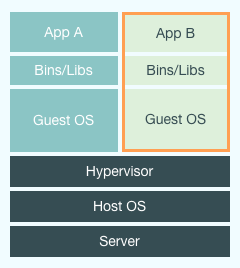
\includegraphics[width=0.45\textwidth]{./images/classic_virtual_machine.png}
    \caption{Klassiche Virtualisierung mit Host OS and Guest OS}
    \label{img:classic_virtual_machine}
  \end{center}
\end{figure}

Ein Linux Container läuft in einem eigenen Prozess im Host Betriebsystem. Der Linux Kernel isoliert
den Prozess von allen anderen Prozessen und mittels Namespaces. Das gibt die Vorteile einer
Virtuallisierung, ist aber viel leichtgewichtiger und Ressourcen schonender, da der Betriebsystem
overhead nur einmal anfällt.

\begin{figure}[htbp]
  \begin{center}
    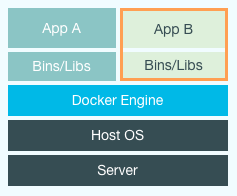
\includegraphics[width=0.45\textwidth]{./images/docker_container.png}
    \caption{Linux Container Virtuallisierung}
    \label{img:docker_container}
  \end{center}
\end{figure}






\cleardoublepage

% ===========================================================================
% Kapitel Paradigmatischer Fall beginns here
% ===========================================================================
  
\chapter{Docker Workflow}\label{chapter:DockerWorkflow}
  
Docker hat den Grunsätzlichen Workflow von Build, Ship, Run. Wie ich das im Proof of Concept
gemacht habe, werde ich hier veranschaulichen.

\section{Build}

Um ein Image zu bauen kann man ein \textit{Dockerfile} erstellen. Das Dockerfile ist wie ein
Script-File, welches die Beschreibung eines Betriebsystems ist. Darin kann angegeben werden
von welchem Docker Image abgeleitet wird. Welche Dateien in dieses Image gepackt werden sollen.
In welchem Benutzerkontext das Image augeführt. Welche Netzwerkports nach aussen hin exposed werden.
Und vieles mehr.

Als zweite Variante kann man ein bestehendes Image starten und live Änderungen am Image vornehmen.
z.B. Konfigurationsdateien anpassen. Mit dem Befehl \textit{docker commit} können dann jegliche
Änderungen in ein neues Image gespeichert werden. Das hat Ähnlichkeit zum bestehenden
Software Entwicklungsprozess, wo man seine Änderungen auch ”committed“.

\subsection{Dockerfile}

Das Dockerfile welches ich für den Proof of Concept erstellt habe, sieht so aus:

\begin{lstlisting}[
  captionpos=b,
  caption=Dockerfile,
  label=Dockerfile
]
  FROM java:8
  MAINTAINER Roman Wuersch

  COPY . /usr/src/yass
  WORKDIR /usr/src/yass

  EXPOSE 9090

  CMD ["./start-in-docker.sh"]
\end{lstlisting}

\begin{description}

\item[Zeile 1] Das Image leitet vom offiziellen OpenJDK 8 Image ab und baut darauf auf.

\item[Zeile 4] Kopiert alle Dateien im aktuellen Pfad ”.“ in das Image in den Pfad ”/urs/src/yass“. Das
sehe ich als eine der grössten Stärken an. Man kann sein Setup Lokal auf seiner Maschine so aufsetzten und testen
bis es alles sauber funktioniert und dann mit dieser Zeile genau den Inhalt in das Image replizieren.

\item[Zeile 5] Setzt das Startverzeichnis

\item[Zeile 7] Gibt an, dass der Port 9090 von einem Prozess verwendet wird und zukünftig angebunden werden kann

\item[Zeile 9] Der Befehl, welcher ausgeführt wird, wenn ein Container aus dem Image gestartet wird.

\end{description}

\subsection{Bauen via Shellscript}

Um das Image zu bauen habe ich ein Shell-Script gemacht:
\\

\begin{lstlisting}[
  captionpos=b,
  caption=Bauen eines Docker Images,
  label=BauenEinesDockerImages
]
#!/usr/bin/env bash
docker rmi -f sushicutta/docker-test
docker build -t sushicutta/docker-test .
\end{lstlisting}

Dieses Shell-Script sucht im aktuellen Verzeichnis ein Dockerfile und baut mit dessen
Angaben das Image.

\begin{description}

\item[Zeile 2] Löscht das bestehende Image sushicutta/docker-test aus dem Docker Hafen

\item[Zeile 3] Erstellt das Image neu anhand der Datei \textit{Dockerfile} unter dem selben Namen.

\end{description}

\section{Ship}

\subsection{Via Docker Hub}

Um das Image zu liefern, kann man nun Docker Hub verwenden.
\\

\begin{lstlisting}[
  captionpos=b,
  caption=Push to Docker Hub,
  label=PushToDockerHub
]
docker push sushicutta/docker-test
\end{lstlisting}

\subsection{Als .tar File}

Oder man kann das Image als .tar Datei speichern.
\\

\begin{lstlisting}[
  captionpos=b,
  caption=Docker Image exportieren,
  label=DockerImageExportieren
]
docker save -o docker-test.tar sushicutta/docker-test
\end{lstlisting}

Das gelieferte Image kann man dann irgendwo wieder importieren.
\\

\begin{lstlisting}[
  captionpos=b,
  caption=Docker Image importieren,
  label=DockerImageImportieren
]
docker load -i docker-test.tar
\end{lstlisting}

\subsection{Via SSH Tunnel}

Oder gleich das Image per SSH transportieren zippen und unzippen on the fly, und mit pv den
Pipe traffic darstellen:
\\

\begin{lstlisting}[
  captionpos=b,
  caption=SSH Transport mit zippen und network traffic Visualisierung,
  label=SSHTransport
]
docker save <image> | bzip2 | pv | \
     ssh user@host 'bunzip2 | docker load'
\end{lstlisting}

\section{Run}

Das Image ist jetzt gebaut worden und im Docker Hafen angekommen, und es trägt den Namen
sushicutta/docker-test.

Dieses Image kann nun beliebig viele Male gestartet werden.

Um das Image zweimal zu starten, benötigt man folgende Commands:
\\

\begin{lstlisting}[
  captionpos=b,
  caption=Image zweimal starten auf den Ports 9091 und 9092,
  label=ImageZweimalStarten
]
docker run -d -p 9091:9090 --name yass-node-1 sushicutta/docker-test
docker run -d -p 9092:9090 --name yass-node-2 sushicutta/docker-test
\end{lstlisting}

Das Image läuft jetzt zweimal, der Inhalt ist zu 100\% identisch. Der unterschied
besteht darin, dass Docker nun den Ports 9091 des Host Betriebsystems auf den Port 9090 des
ersten Containers mapped und analog den Port 9092 des Host Betriebsystems auf den Port 9090
des zweiten Containers.

\begin{figure}[htbp]
  \begin{center}
    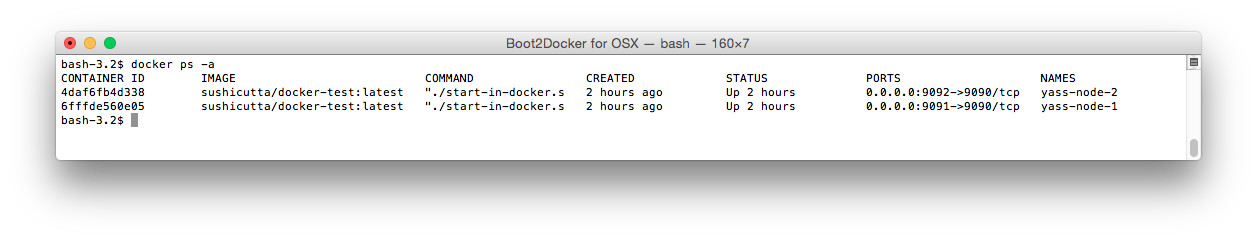
\includegraphics[width=1.0\textwidth]{./images/twoProcesses.png}
    \caption{Zwei identische Container auf verschiedenen Ports}
    \label{img:twoProcesses}
  \end{center}
\end{figure}

Was jetzt noch zum trägen kommt, ist der Start Befehl, der im Dockerfile
konfiguriert wurde. In unserem Beispiel start-in-docker.sh:
\\

\begin{lstlisting}[
  captionpos=b,
  caption=Start Script im Docker Container,
  label=StartScriptImDockerContainer
]
#!/usr/bin/env bash
java -Dfile.encoding=UTF-8 -classpath \
  "/usr/src/yass/lib/*:/usr/src/yass/build/classes/tutorial"\
  ch.softappeal.yass.tutorial.server.web.JettyServer 2>&1
\end{lstlisting}

Den Output der Prozesse kann man mit dem Befehl docker logs anschauen.

\begin{figure}[htbp]
  \begin{center}
    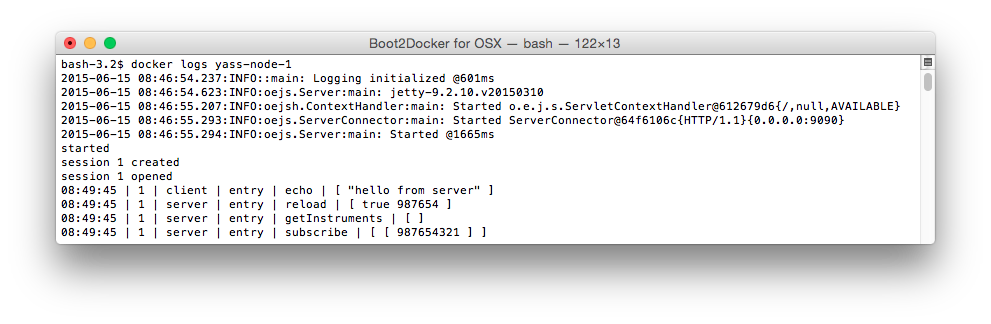
\includegraphics[width=1.0\textwidth]{./images/logOutput.png}
    \caption{Output am Stdout und Stderr sichtbar machen vom Host Betriebsystem}
    \label{img:logOutput}
  \end{center}
\end{figure}







\cleardoublepage

% ===========================================================================
% Anhang beginns here
% ===========================================================================

\appendix

\pagenumbering{alph}

% ===========================================================================
% Abbildungsverzeichnis beginns here
% ===========================================================================

\listoffigures

\cleardoublepage

% ===========================================================================
% Literaturverzeichnis beginns here
% ===========================================================================
  
\chapter{Literaturverzeichnis}\label{chapter:Literaturverzeichnis}





\cleardoublepage

\end{document}
